\section{Empirical Evaluation and Analysis}

\begin{table*}[t]
\centering
\caption{Comparative Performance Metrics Across Selected Experimental Sweeps}
\label{tab:results}
\noindent\resizebox{\textwidth}{!}{%
\begin{tabular}{lllcrcrcccr}
\toprule
Experiment ID & Policy & DA Mode & Workload & Avg. Size & TPS & Latency (s) & Fairness & L1 Gas/Tx & Prove Time (s) & Cost/Tx (USD) \\
\midrule
\texttt{baseline} & FCFS & Calldata & Steady & 36.80 & 19.83 & 7.03 & 0.75 & 21,423.88 & 0.00 & \$0.194 \\
\texttt{s3\_pol\_fcfs} & FCFS & Calldata & Steady & 36.84 & 19.85 & 7.02 & 0.75 & 20,744.35 & 0.00 & \$0.188 \\
\texttt{s3\_pol\_feepriority} & FeePriority & Calldata & Steady & 37.07 & 19.98 & 7.02 & 0.76 & 111,964.07 & 0.00 & \$0.007 \\
\texttt{s3\_burst\_feepriority} & FeePriority & Calldata & Burst & 50.83 & 29.09 & 7.02 & 0.74 & 111,986.50 & 0.00 & \$0.007 \\
\texttt{s3\_burst\_timeboost} & TimeBoost & Calldata & Burst & 50.01 & 29.45 & 7.02 & 0.77 & 111,995.20 & 0.00 & \$0.007 \\
\texttt{s4\_da\_blob} & FCFS & Blob & Steady & 36.94 & 19.91 & 7.02 & 0.76 & 4,596.32 & 0.00 & \$0.057 \\
\texttt{s4\_da\_offchain} & FCFS & Offchain & Steady & 36.81 & 19.84 & 7.02 & 0.75 & 3,615.49 & 0.00 & \$0.033 \\
\texttt{s5\_real\_bs\_0050} & FCFS & Calldata & Steady & 42.17 & 5.06 & 7.03 & 0.80 & 24,594.02 & 317.82 & \$0.184 \\
\texttt{s5\_real\_bs\_0500} & FCFS & Calldata & Steady & 246.00 & 4.92 & 7.06 & 0.98 & 19,502.72 & 1487.31 & \$0.146 \\
\bottomrule
\end{tabular}%
}
\end{table*}

\subsection{Stage 1: Fixed Batching and Aggregation Anomalies}
Stage 1 sweeps evaluate fixed batching by varying target batch sizes ($B_{\text{max}} \in [25, 1000]$) and timeouts ($T_{\text{timeout}} \in [500, 10000]$ ms) under a stable 25 TPS Poisson workload.
The results confirm the expected latency-cost trade-off: larger batch sizes reduce per-transaction L1 gas costs by amortizing the fixed batch submission overhead, but increase mempool queueing delay. We model the average queue wait time as:
\begin{equation}
W_q \approx \frac{1}{2} \min\left(T_{\text{timeout}}, \frac{B_{\text{max}}}{\lambda}\right)
\end{equation}
This model matches the empirical FCFS latencies: a short 500~ms timeout (\texttt{s1\_to\_00500}) achieves a low L2-to-L1 latency of 7019.70~ms, but inflates costs to 23,549.75 gas/tx because batches are sealed before they can fill. Conversely, a 10000~ms timeout (\texttt{s1\_to\_10000}) reduces gas costs to 19,681.09 gas/tx but increases latency to 7033.44~ms. Similarly, scaling batch size from 25 (\texttt{s1\_bs\_0025}) to 500 (\texttt{s1\_bs\_0500}) amortizes fixed L1 overhead, reducing costs from 20,550 gas/tx to 19,482 gas/tx, while latency increases from 7023~ms to 7059~ms.
\begin{figure}[htbp]
\centering
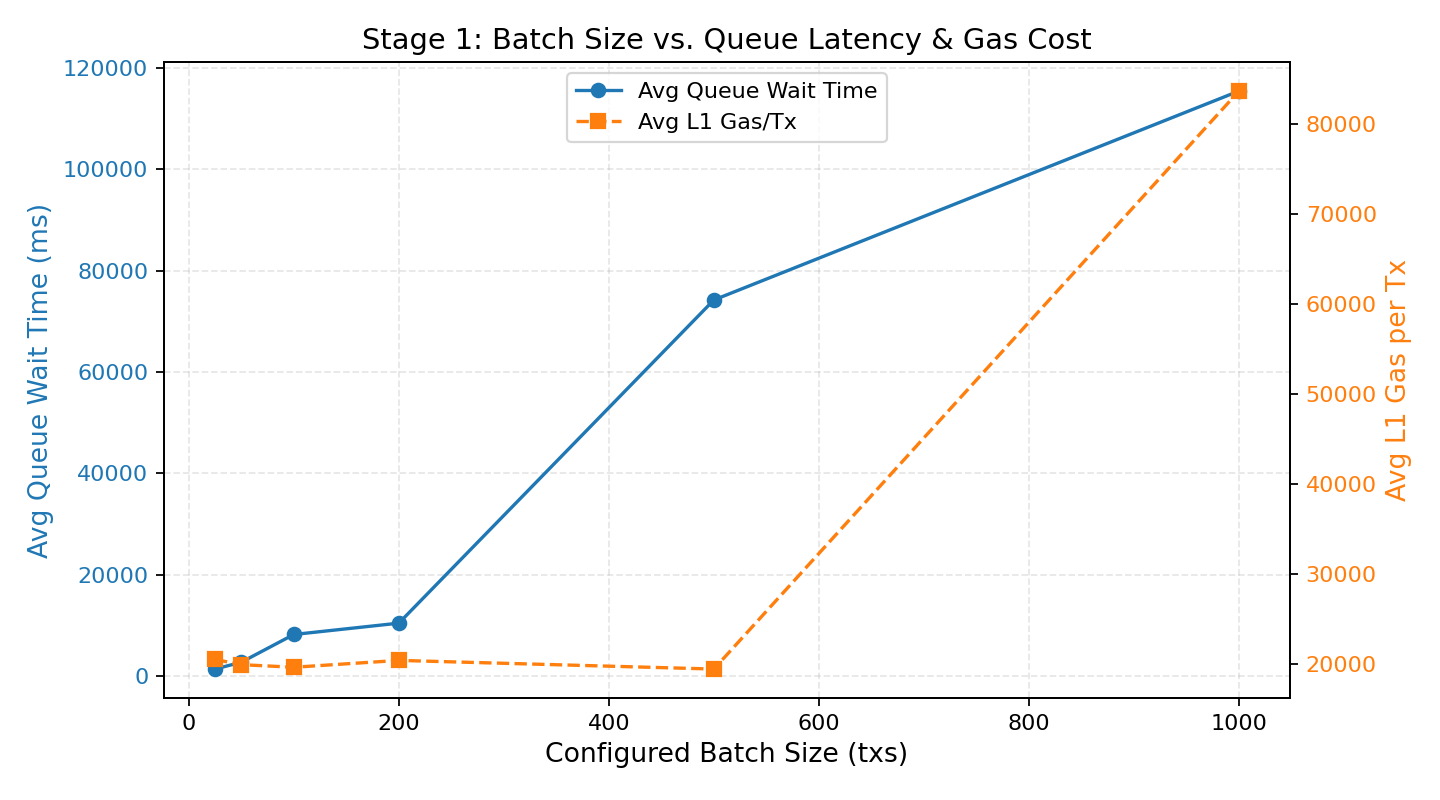
\includegraphics[width=\linewidth]{figures/s1_batch_size_vs_latency_gas.png}
\caption{Stage 1: L1 Gas Cost per Transaction vs. Average L2-to-L1 Finalization Latency under Varying Batch Sizes.}
\label{fig:s1_batch_size}
\end{figure}

We identified a critical **metrics aggregation bug** in the benchmark execution. For the 1000 batch size configuration (\texttt{s1\_bs\_1000}), the system reported a gas cost of 83,626.43 gas/tx (a 307.6\% increase). In reality, the test generated 3,332 transactions across 6 batches. Two batches were full (605 and 661 transactions, sealed early due to L1 gas limits), one had 1 transaction, and three were empty. To avoid division-by-zero, the metrics script replaced \texttt{tx\_count} = 0 with \texttt{max(tx\_count, 1)}. Since submitting any batch to L1 carries a fixed cost of $\sim$112,000 gas, the script treated the three empty batches as containing 1 transaction that consumed 112,000 gas, heavily skewing the unweighted arithmetic average of batch means. The volume-weighted average (total gas divided by total transactions) was actually **19,771.15 gas/tx**, showing that unweighted averages introduce severe boundary distortions.

\subsection{Stage 2: Adaptive Batching and the Hysteresis Trap}
Stage 2 evaluates dynamic batch size adjustments under varying traffic rates. Under bursty traffic, the adaptive policy (\texttt{s2\_adaptive\_burst}) dynamically scales batch sizes to backlog depth, outperforming the fixed policy (\texttt{s2\_fixed\_burst}) on all fronts: committed throughput rises to **29.31 TPS** (vs. 29.09 TPS), gas cost drops to **21,046.18 gas/tx** (vs. 21,081.18 gas/tx), and Jain's Fairness Index increases to **0.769** (vs. 0.753). By using smaller batches during idle periods and scaling up during bursts, the adaptive policy maintains low latency without sacrificing gas amortization.

However, we identified a mathematical design flaw in the sealing logic under steady load, which we term the **Hysteresis Threshold Trap**. For the sequencer to seal at the small batch size $S_b$, the mempool pending count $P$ must satisfy $S_b \le P < L_t$, where $L_t$ is the low-load threshold. The system configurations violate this (e.g., $S_b = 50, L_t = 50$). Under low load, the target is $S_b$, but since $P < L_t \le S_b$, the pending count can never reach $S_b$ to trigger a size-based seal. Once $P$ reaches $L_t$, the target instantly jumps to the medium size ($M_b = 100$). The sequencer can never seal at $S_b$, and the adaptive policy collapses into a fixed-batching policy at the larger batch size.

\subsection{Stage 3: Sequencer Scheduling and Nonce Reordering}
Stage 3 sweeps evaluate FCFS, FairBFT, FeePriority, TimeBoost, and BlobPacking scheduling policies. The empirical data reveals a catastrophic **Nonce Reordering Vulnerability** in all priority-based scheduling policies (\texttt{FeePriority}, \texttt{TimeBoost}, and \texttt{BlobPacking}) under single-account workloads:
\begin{itemize}
    \item \textbf{Silent Transaction Drops:} For these three policies, **96 out of 97 submitted batches were completely empty**. Only 2 transactions successfully executed in the entire 180-second benchmark run.
    \item \textbf{Gas Inflation:} Due to the empty-batch metrics bug, the reported gas per transaction inflated to **$\sim$111,964 gas**, whereas the true gas per transaction for the two executed transactions was **5,467,233 gas** (amortizing 97 L1 batch submissions over only 2 transactions).
\end{itemize}
In account-based networks like the EVM, transactions from a single sender must execute sequentially in strict nonce order. Policies like FeePriority and TimeBoost reorder transactions by fee bids. If a sender submits transaction $N$ with a low fee and $N+1$ with a high fee, the sequencer places $N+1$ before $N$ in the batch. The executor's state transition function rejects $N+1$ due to a nonce gap, stalling the sender's account nonce. Because the workload generator used a single sender account (\texttt{0xf39fd6e...}), this nonce violation at the beginning of Batch 2 caused the executor to silently reject 100\% of transactions in all subsequent batches. The system marked these runs as PASS because empty proofs were successfully verified on L1, masking the total execution failure.

Under burst workloads, **TimeBoost** achieved the highest Jain's Fairness Index (\(0.77\)) compared to FCFS (\(0.75\)) and FeePriority (\(0.74\)). By grouping transactions into 5-second windows and only allowing priority bidding within each window, TimeBoost prevents new high-fee transactions from starving older, low-fee transactions.
\begin{figure}[htbp]
\centering
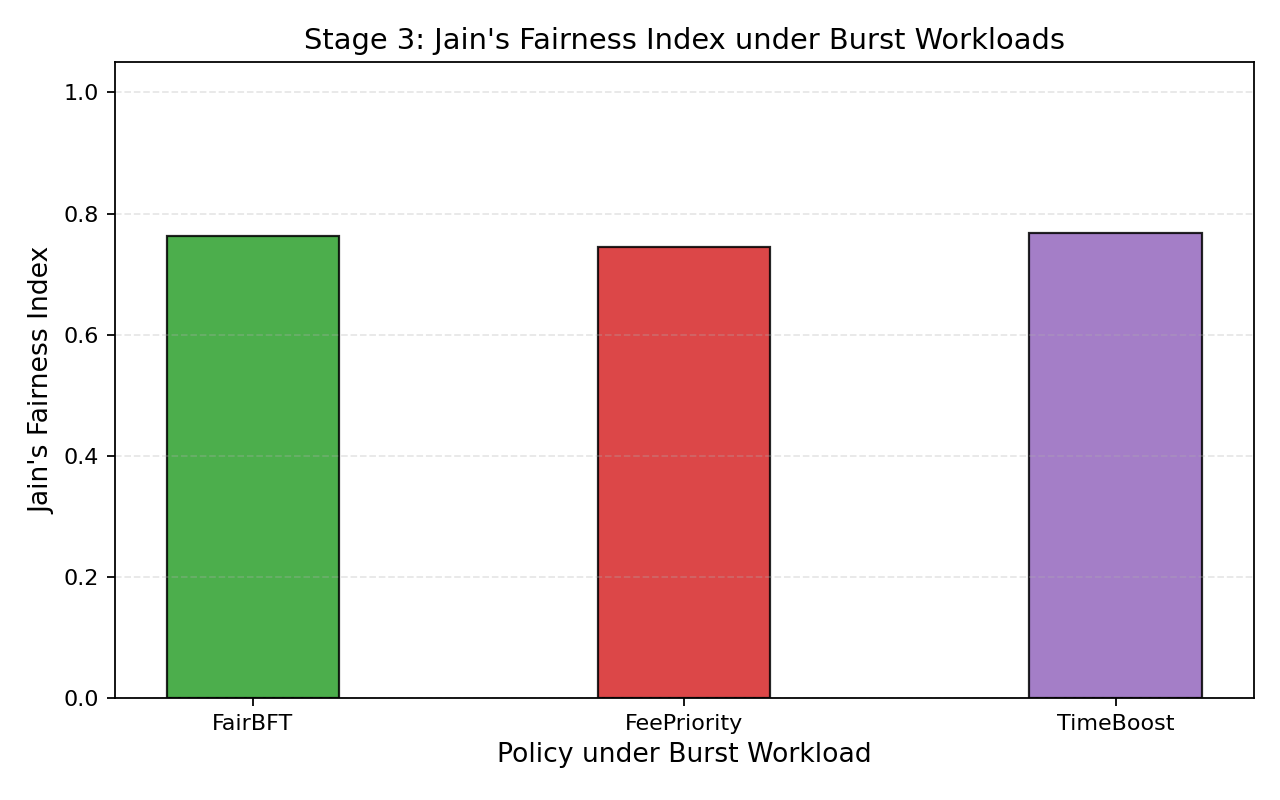
\includegraphics[width=\linewidth]{figures/s3_jains_fairness_burst.png}
\caption{Stage 3: Jain's Fairness Index for FCFS, FeePriority, and TimeBoost Scheduling Policies under Bursty Workloads.}
\label{fig:s3_fairness}
\end{figure}

\subsection{Stage 4: Data Availability Modes and Blob Sealing}
Stage 4 evaluates L1 calldata, EIP-4844 blobs, and off-chain data availability (DA). The results demonstrate massive L1 cost reductions under Blob and Off-chain DA (see Table~\ref{tab:results}):
\begin{itemize}
    \item \textbf{Calldata DA (\texttt{s4\_da\_calldata}):} Average cost of **\$0.188 per transaction** (20,739 gas/tx).
    \item \textbf{Blob DA (\texttt{s4\_da\_blob}):} Average cost of **\$0.057 per transaction** (4,596 gas/tx)---a **78.5\% cost saving**.
    \item \textbf{Off-chain DA (\texttt{s4\_da\_offchain}):} Average cost of **\$0.033 per transaction** (3,615 gas/tx)---an **83.1\% cost saving**.
    \item \textbf{Optimal Blob DA (\texttt{s4\_blob\_fill\_095}):} Under 95\% blob capacity utilization, the cost per transaction drops to **2,602 gas/tx** (an **87.8\% cost saving** over calldata).
\end{itemize}
\begin{figure}[htbp]
\centering

\includegraphics[width=\linewidth]{s4_da_mode_efficiency}
\caption{Stage 4: Amortized Gas Consumption per Transaction across Calldata, EIP-4844 Blob, and Off-chain Data Availability (DA) Modes.}
\label{fig:s4_da}
\end{figure}
However, in low-throughput settings, the time-driven FCFS sequencer seals batches before accumulating enough data, posting partially empty blobs ($\sim$17.8~KB out of 120~KB) and diluting blob utilization. Furthermore, the sequencer's sealing engine completely ignores the \texttt{blob\_fill\_target} configuration parameter in the code, representing a dead config parameter.

\subsection{Stage 5: zkVM Prover Scaling and Economics}
Stage 5 profiles the RISC0 zkVM prover backend using Groth16 proof generation. The results show that ZK proof generation is the primary system bottleneck, scaling non-linearly with batch size:
\begin{itemize}
    \item \textbf{Batch size 50 (\texttt{s5\_real\_bs\_0050}):} Prover time is **317.8 seconds** ($\approx$5.3 minutes) per proof.
    \item \textbf{Batch size 100 (\texttt{s5\_real\_bs\_0100}):} Prover time is **540.8 seconds** ($\approx$9.0 minutes) per proof.
    \item \textbf{Batch size 200 (\texttt{s5\_real\_bs\_0200}):} Prover time is **782.4 seconds** ($\approx$13.0 minutes) per proof.
    \item \textbf{Batch size 500 (\texttt{s5\_real\_bs\_0500}):} Prover time explodes to **1,487.3 seconds** (**24.8 minutes**).
\end{itemize}
\begin{figure}[htbp]
\centering

\includegraphics[width=\linewidth]{figures/s5_prover_time_vs_batch_size.png}
\caption{Stage 5: RISC0 zkVM Proving Time (seconds) as a Function of Target Batch Size, demonstrating step-function scaling.}
\label{fig:s5_prover}
\end{figure}
Proving time scales as a step-function governed by cycle-based segment boundaries ($2^{20}$ cycles per segment). Merkle root updates and transaction signature verification inside the zkVM represent the bulk of this computing cost. Even at a low workload of 5 TPS (generating 250 transactions in 50 seconds), the sequencer produces 5 batches of size 50. Generating proofs for these batches requires **1,589 seconds** ($\approx$26.5 minutes) of cumulative prover time. Without parallel proving, a single prover creates a massive queue backlog, limiting the committed TPS to $\sim$5 TPS and delaying L2-to-L1 hard finality by up to 25 minutes.

We perform a linear regression on wall-clock proving time $T(N)$ as a function of batch size $N$:
\begin{equation}
T(N) = A + B \times N
\end{equation}
where the Fixed SNARK Compression Setup ($A$) is 70--80 seconds, and the Marginal Proving Cost ($B$) is $\approx$5.7 seconds per transaction. Amortizing the fixed SNARK setup reduces the proving time per transaction from 7.5s (at size 50) to 6.0s (at size 246).

Similarly, L1 gas per batch is modeled as $\text{L1 Gas}(N) = F + M \times N$, where the Fixed L1 Verifier Overhead ($F$) is 30,000--50,000 gas and the Marginal L1 Cost ($M$) is $\approx$19,300 gas. As batch size increases, the per-transaction gas decays asymptotically towards $M$.